\input{../documents-common/preamble.tex}
\usepackage[framed]{mcode}
%\usepackage{listings} % Include the listings-package
\begin{document}
\maketitle[Finite Element Methods]{Assignment 2}

\section{}
\subsection{Derivation}
Start with variational form of Poisson's Equation by Multiplying $f = -\Delta u$ by $v$ and integrating over $\Omega$:
\begin{align}
  -\int_\Omega -\Delta uv\,\d x = \int_\Omega fv\,\d x
\end{align}
And then use Green's Theorem (specifically, equation 4.3 from the book) and simplify to find:
\begin{align}
  -\int_\Omega -\Delta uv\,\d x &= \int_\Omega fv\,\d x\nn
  \int_\Omega \nabla u\cdot\nabla v\,\d x - \int_{\partial\Omega} n\cdot\nabla u v\,\d s &= \int_\Omega fv\,\d x\nn
  \int_\Omega \nabla u\cdot\nabla v\,\d x &= \int_\Omega fv\,\d x.
\end{align}
Here $v$ are members of the standard space $V_0$, $ V = \left\{v: \norm{v}_{L^2(\Omega)}+\norm{\nabla v}_{L^2(\Omega)}<\infty\right\}, V_0 =  \left\{ v\in V : v|_{\partial\Omega} = 0\right}$.
We now further restric us to the space $V_h$ of continous piecewise linears on triangulation $K$ (with $V_{h,0}$ defined similarlly to $V_0$) then the FEM formulation is:
\begin{align}
\int_\Omega \nabla u_h\cdot\nabla v\,\d x &= \int_\Omega fv\,\d x,\; \forall v \in V_{h,0}.
\end{align}
now let the set of $\phi_i,\, i = 1,\ldots,n$ (where $n$ is the number of interior nodes) define a basis of $V_{h,0}$, then the above equation has to hold for all $\phi_i$, that is
\begin{align}
\int_\Omega \nabla u_h\cdot\nabla \phi_i\,\d x &= \int_\Omega f\phi_i\,\d x,\; i = 1,\ldots,n.
\end{align}
Since $u_h \in V_{h,0}$ we can write
\begin{align}
  u_h = \sum_{j=1}^{n} \alpha_j \phi_j,
\end{align}
inserting this into the previous equation we find
\begin{align}
  \sum_{j=1}^{n}\alpha_j\int_\Omega \nabla \phi_j\cdot\nabla \phi_i\,\d x &= \int_\Omega f\phi_i\,\d x,\; i = 1,\ldots,n.
\end{align}
Which can be written as $A\alpha = b$.
\par We have implemented this equation in Matlab (using the implementation details discussed in lab 2). We construct our $A$ matrix and $b$ vector as:
\lstinputlisting{./code/assemble.m}
with the helper function
\lstinputlisting{./code/create_AK_bK.m}

\subsection{Results}
We have computed the Galerkin results, the exact solution, and the error with $f(\vec x) = 8\pi^2\sin(2\pi x_1)\sin(2\pi x_2)$ and $h = 1/8$ and $h = 1/16$ in figure \ref{fig:1_sol}, \ref{fig:1_exact}, and \ref{fig:1_err}

\begin{figure}[!Hh]
\centering
\begin{minipage}{.5\textwidth}
  \centering
  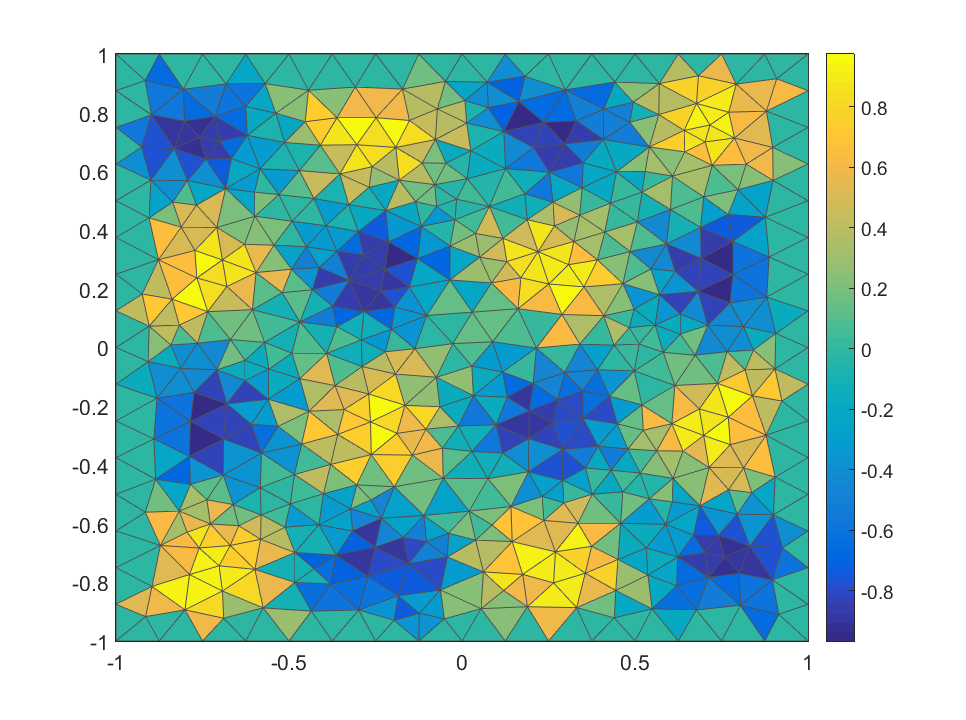
\includegraphics[width=\linewidth]{./plots/01_1_8_sol}
\end{minipage}%
\begin{minipage}{.5\textwidth}
  \centering
  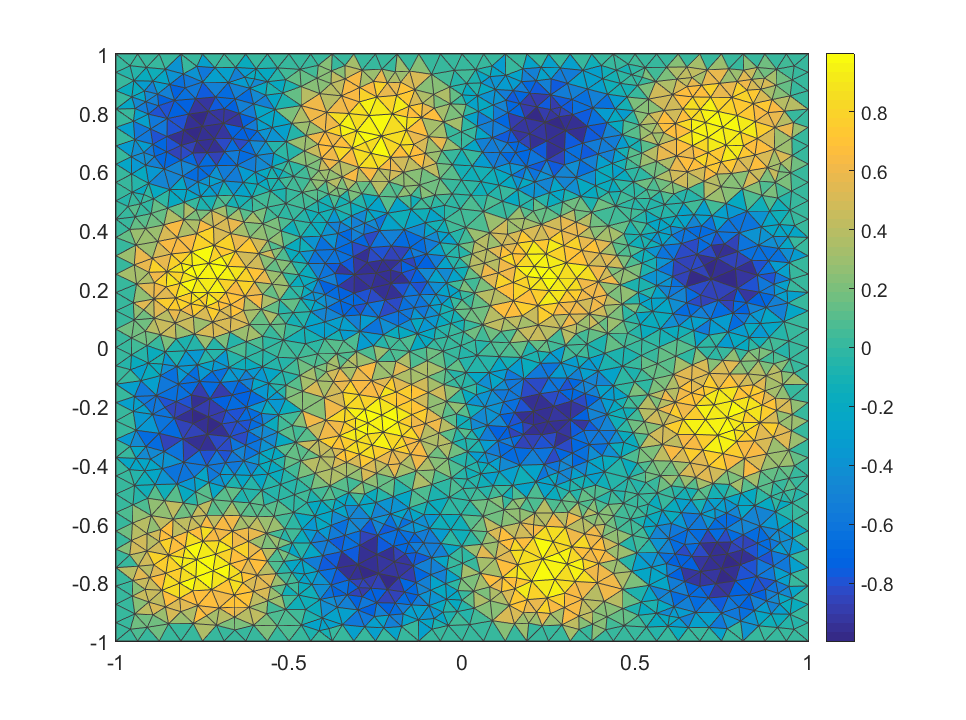
\includegraphics[width=\linewidth]{./plots/01_1_16_sol}
\end{minipage}
\caption{The Galerkin solution}
\label{fig:1_sol}
\end{figure}

\begin{figure}[!Hh]
\centering
\begin{minipage}{.5\textwidth}
  \centering
  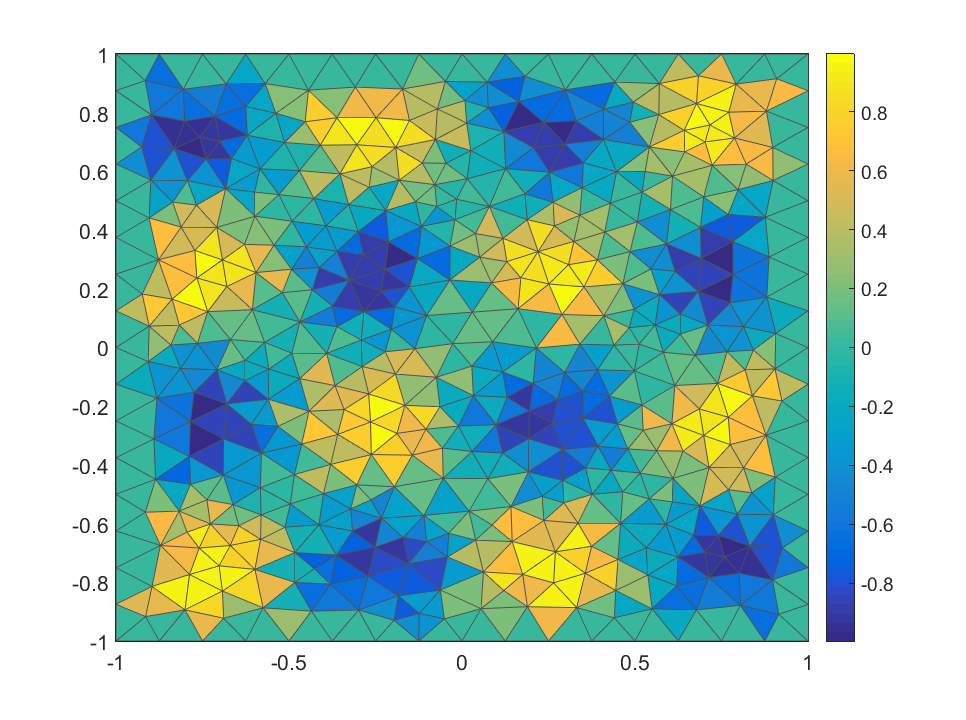
\includegraphics[width=\linewidth]{./plots/01_1_8_exact}
\end{minipage}%
\begin{minipage}{.5\textwidth}
  \centering
  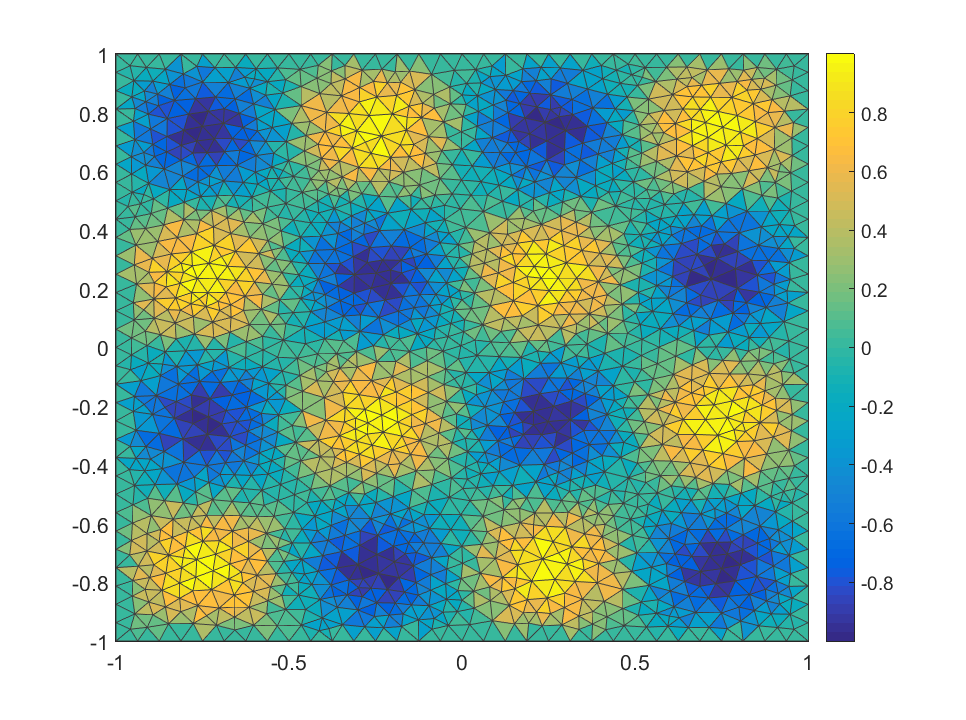
\includegraphics[width=\linewidth]{./plots/01_1_16_exact}
\end{minipage}
\caption{The exact solution}
\label{fig:1_exact}
\end{figure}

\begin{figure}[!Hh]
\centering
\begin{minipage}{.5\textwidth}
  \centering
  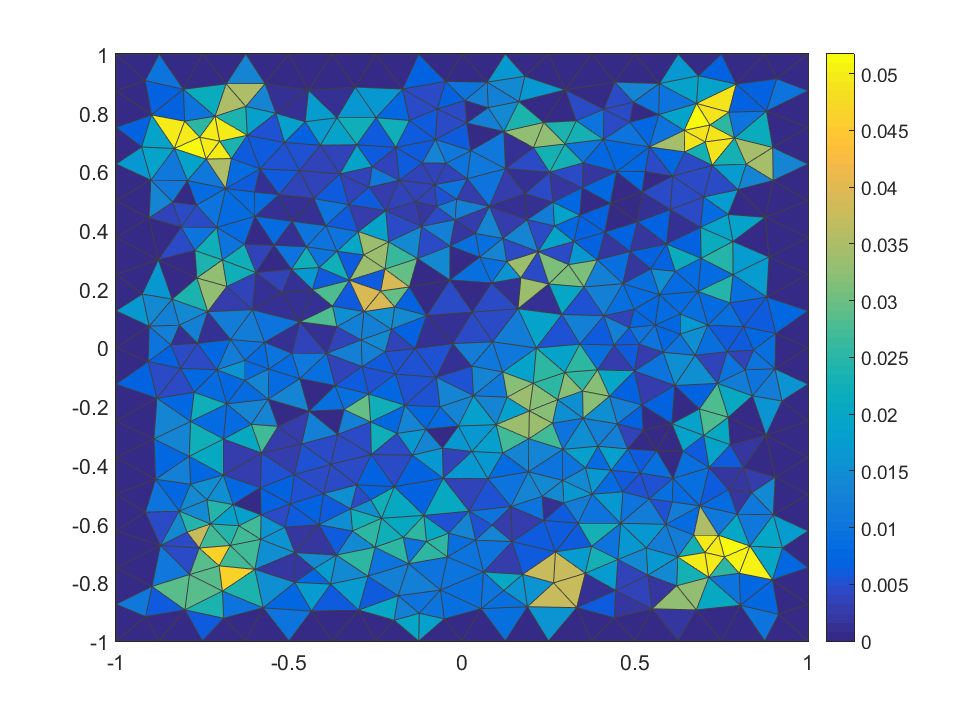
\includegraphics[width=\linewidth]{./plots/01_1_8_err}
\end{minipage}%
\begin{minipage}{.5\textwidth}
  \centering
  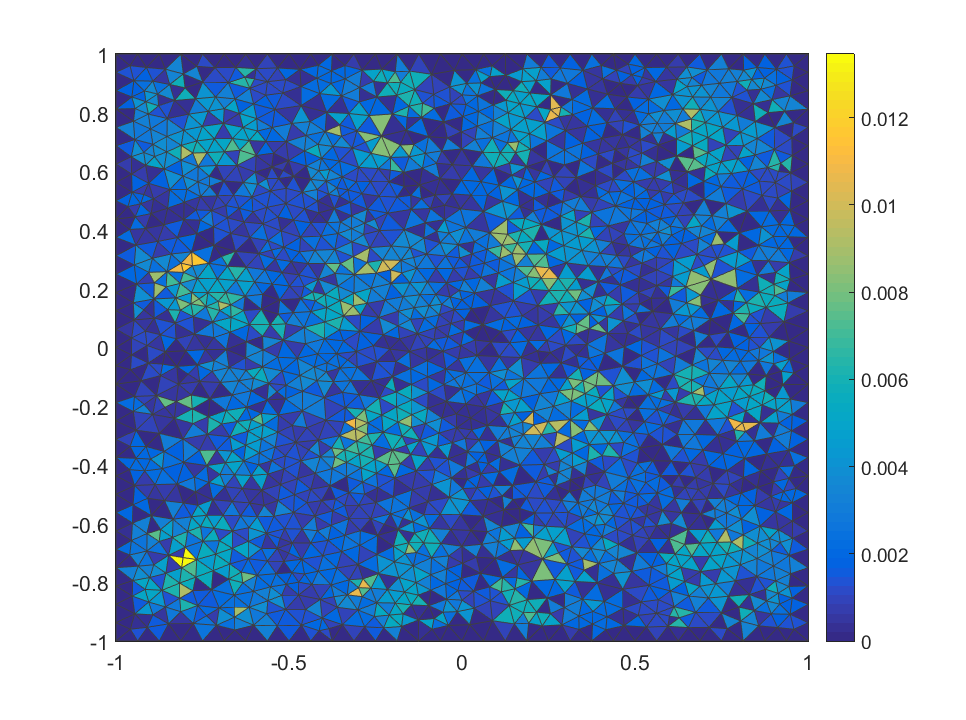
\includegraphics[width=\linewidth]{./plots/01_1_16_err}
\end{minipage}
\caption{The absolute difference between the Galerkin and exact solution}
\label{fig:1_err}
\end{figure}

\subsection{convergence}
We have determined the convergence rate in the energy norm of the error $\norm{u-U}_E^2$  for various values of $h_\text{max}$  between $1/2$ and $1/32$, and the fitting a linear function to $\log \norm{u-U}_E^2$ over $\log_2 h_\text{max}$. The order of convergence is then given by the slope of the fit (as $\log x^a = a\log x$). We find an order of $\approx 0.84$. The results are plotted in \ref{fig:1_convergence}.
\begin{figure}[!Hh]
  \centering
  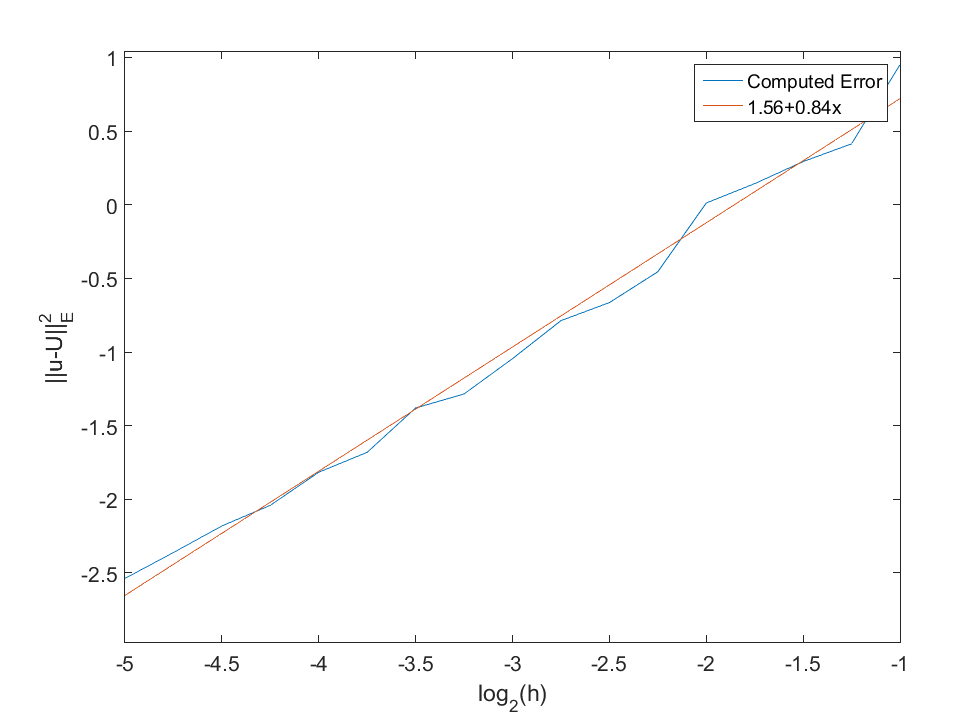
\includegraphics[width=\textwidth]{./plots/01_convergence}
  \caption{Convergence plot of our Galerkin plot.}
  \label{fig:1_convergence}
\end{figure}

\newpage
\section{}
\subsection{Galerkin Formulation}
The variational formulation for our problem is
\begin{align}
  \int_\Omega fv\,\dx &= \int_\Omega \left(\partial_t u + \beta\cdot\nabla u - \nabla\cdot\left(\epsilon\nabla u\right)\right)v\,\d x\nn
  &=\int_\Omega \left(\partial_t u + \beta\cdot\nabla u + \epsilon\nabla u \cdot \nabla\right) v\,\d x - \int_{\partial\Omega}\left(\epsilon\nabla u \cdot \vec n\right)v\,\d s\nn
  &=\int_\Omega \left(\partial_t u + \beta\cdot\nabla u + \epsilon\nabla u \cdot \nabla\right)v\,\d x\nn
\end{align}
here the last step follows from the fact the $v \in V_{h,0}$ and is therefore 0 along the boundary (which we have chosen as a boundary condition).
Now we replace $u$ with $u_h$ and write both $u_h$ and $v$ in terms of the basis functions $\phi$ again, giving:
\begin{align}
  \int_\Omega f\phi_i\,\d x &= \alpha_j\int_\Omega\left(\epsilon \nabla\phi_j\cdot\nabla\phi_i +\beta\cdot\nabla \phi_j\phi_i\right)\,\d x + \dot \alpha_j\int_\Omega \phi_i\phi_j\,\d x\nn
  \vec b &= A \vec \alpha + B \dot{\vec \alpha}
\end{align}
Now, noting that $\dot{\vec \alpha} = B^{-1}\left(\vec b - \epsilon A \vec \alpha\right)$, we apply time discretization using the Crank-Nicolson scheme:
\begin{align}
&\frac{\alpha^+-\alpha}{\Delta t} = \frac{1}{2}\left(\dot\alpha^++\dot\alpha\right)\nn
&\implies \left(B+\frac{\Delta t}{2}A\right)\alpha^+ = \left(B-\frac{\Delta t}{2}A\right)\alpha+\frac{\Delta t}{2}b
\end{align}
\end{document}
